\section{The source complex and the one-pleat seam}\label{sec:source}
We now leave the rotational-radial class.  It suffices to construct the case $R=1$; scaling source and target by $R$ then multiplies volume by $R^3$.

Let $H$ be the regular decagon inscribed in the unit circle, with outer vertices
\[
o_k=(\cos(2\pi k/10),\sin(2\pi k/10)),\qquad k=0,\ldots,9.
\]
Set
\[
\rho=\frac{13}{20},\qquad i_k=\rho o_k,
\]
and let $z=(0,0)$ be the center.  Triangulate $H$ by the $30$ triangles
\begin{align*}
&(z,i_k,i_{k+1}),\\
&(i_k,o_k,o_{k+1}),\\
&(i_k,o_{k+1},i_{k+1}),
\end{align*}
with indices modulo $10$.  All squared source lengths lie in $\mathbb Q(\sqrt5)$.

The ten outer vertices are identified in cyclic order as
\begin{equation}\label{eq:boundarywords}
A_2,\ A_1,\ J,\ C,\ J,\ B_1,\ B_2,\ B_1,\ J,\ A_1.
\end{equation}
Thus the boundary traces the graph
\[
A_2-A_1-J-C-J-B_1-B_2-B_1-J-A_1-A_2.
\]
Every seam edge is traversed twice in opposite directions, and the branch $J-C-J$ is the single pleat.  The ten inner vertices and the center remain distinct.  Hence the quotient has $17$ vertices.

\begin{figure}[t]
\centering
\includegraphics[width=.92\textwidth]{figures/construction_multiview.pdf}
\caption{The source triangulation and four opaque views of the certified target surface.  Red edges indicate the seam graph; the points $C$ and $J$ are marked in the target views.  In particular, the opposite, near-side, and top views make clear that $C$ is a vertex of the polyhedral surface, not an interior point.  The drawings are for visualization only; the proof uses the exact coordinates in \cref{sec:coordinates}.}
\label{fig:construction}
\end{figure}

\begin{figure}[H]
\centering
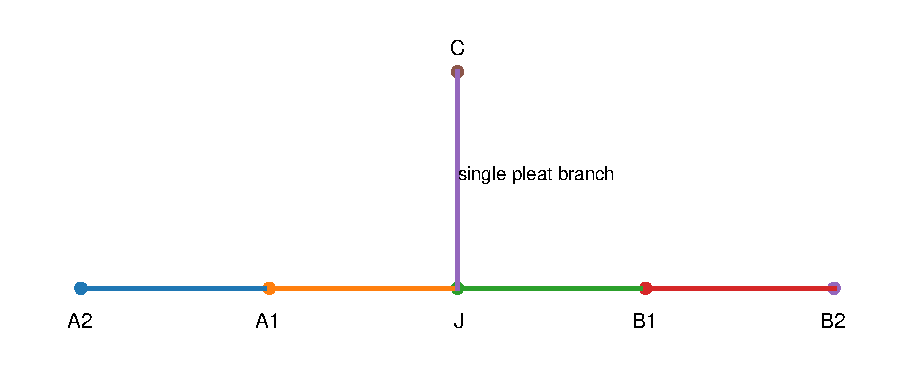
\includegraphics[width=.50\textwidth]{figures/seam_graph.pdf}
\caption{Combinatorial seam graph.  The branch $JC$ is the single pleat.  The actual target coordinates are not coplanar and are listed in \cref{sec:coordinates}.}
\label{fig:seam}
\end{figure}

\section{Explicit target coordinates}\label{sec:coordinates}
Let
\[
\lambda=\frac{99999}{100000}.
\]
Each target vertex is $\lambda$ times the finite-decimal vector in \cref{tab:coords}.  Every displayed decimal is interpreted as an exact rational number.  The affine image of each source triangle is determined by the images of its three vertices.

\begin{table}[H]
\centering
\small
\caption{Base target coordinates before multiplication by $\lambda=99999/100000$.}
\label{tab:coords}
\begin{tabular}{@{}lrrr@{}}
\toprule
vertex & $x$ & $y$ & $z$\\
\midrule
$J$ & 0.114996453431 & 0.652042463578 & 0.359274110539\\
$A_1$ & 0.713527595885 & 0.556758865942 & 0.238247176413\\
$A_2$ & 0.904510611077 & 0.150919970833 & -0.186942534628\\
$B_1$ & -0.269259146678 & 0.427202794161 & 0.787947375499\\
$B_2$ & -0.411232941130 & -0.173302559313 & 0.822628398965\\
$C$ & -0.407447365206 & 0.632905197995 & 0.029649729336\\
$z$ & 0 & 0 & 0\\
$I_0$ & 0.650000000000 & 0 & 0\\
$I_1$ & 0.525861046344 & 0.382060413990 & 0\\
$I_2$ & 0.201227167335 & 0.617682813279 & 0.021807551587\\
$I_3$ & -0.138361314859 & 0.605243587298 & -0.192448295874\\
$I_4$ & -0.192247060016 & 0.586039489637 & 0.205179883277\\
$I_5$ & -0.332154604650 & 0.312020954927 & 0.463482731389\\
$I_6$ & -0.424437564120 & -0.078307526511 & 0.486025395896\\
$I_7$ & -0.126467920004 & 0.156558885543 & 0.618057586773\\
$I_8$ & 0.208351084601 & 0.348929212409 & 0.507285156764\\
$I_9$ & 0.525861046344 & 0.263795278601 & 0.276373318043\\
\bottomrule
\end{tabular}
\end{table}

Let $g:H\to\R^3$ denote the resulting continuous piecewise-affine map.  Continuity holds because adjacent triangles use the same target coordinates on their common vertices, including the identifications in \eqref{eq:boundarywords}.

\section{Exact certification}\label{sec:certificate}
We now establish the geometric properties of $g$.  All sign and intersection assertions in this section are checked by exact arithmetic in the supplied programs; the verification methods are described explicitly so that the certificate is finite and reproducible.

\subsection{Strict nonexpansion on every triangle}
For a source triangle choose two edge vectors $u,v$ from a common vertex and set
\[
S=\begin{pmatrix}
\langle u,u\rangle & \langle u,v\rangle\\
\langle u,v\rangle & \langle v,v\rangle
\end{pmatrix}.
\]
Let $T$ be the corresponding Gram matrix of the target edge vectors.  A tangent vector with coordinate column $\xi\in\R^2$ has squared source length $\xi^TS\xi$ and squared target length $\xi^TT\xi$.  Thus the affine triangle map is strictly nonexpansive if
\[
S-T\succ0.
\]

\begin{lemma}\label[lemma]{lem:lip}
For each of the $30$ source triangles, $S-T$ is positive definite.  Hence $g$ is $1$-Lipschitz on $H$.
\end{lemma}

\begin{proof}
For a real symmetric $2\times2$ matrix, positive definiteness is equivalent to positivity of the two diagonal entries and of the determinant.  The verifier computes, for each triangle,
\[
(S-T)_{11}>0,\qquad (S-T)_{22}>0,\qquad \det(S-T)>0.
\]
The source terms lie in $\mathbb Q(\sqrt5)$ and the target terms are rational; signs in $\mathbb Q(\sqrt5)$ are reduced to rational comparisons by squaring only after the signs of the rational coefficients are known.  Thus no floating-point sign decision is used.

To pass from triangles to the whole decagon, take $x,y\in H$.  Convexity of $H$ implies that the segment $[x,y]$ remains in $H$ and crosses finitely many source triangles.  On each subsegment the image curve has length at most the source subsegment length.  Summing yields
\[
|g(x)-g(y)|\le \operatorname{length}(g([x,y]))\le |x-y|.
\]
\end{proof}

\subsection{The quotient is a sphere}
\begin{lemma}\label[lemma]{lem:sphere}
The quotient triangulation is a connected closed orientable triangulated $2$-manifold with
\[
V=17,\qquad E=45,\qquad F=30,
\]
and hence is topologically $S^2$.
\end{lemma}

\begin{proof}
The exact combinatorial verifier checks that every edge belongs to exactly two faces, every vertex link is one cycle, the complex is connected, and the listed face orientations agree oppositely along each shared edge.  Hence it is a connected closed orientable $2$-manifold.  Its Euler characteristic is
\[
17-45+30=2,
\]
so the classification of closed orientable surfaces gives $S^2$.
\end{proof}

\subsection{No unintended triangle intersections}
\begin{lemma}\label[lemma]{lem:embedded}
The geometric realization of the quotient complex is embedded in $\R^3$.
\end{lemma}

\begin{proof}
There are $\binom{30}{2}=435$ unordered face pairs.  The independent verifier tests intersection by solving exactly
\[
A_0+\alpha(A_1-A_0)+\beta(A_2-A_0)
=
B_0+\gamma(B_1-B_0)+\delta(B_2-B_0)
\]
under the barycentric inequalities
\[
\alpha,\beta,1-\alpha-\beta,\gamma,\delta,1-\gamma-\delta\ge0.
\]
The three coordinate equations have rank $3$ in every tested pair, leaving one affine parameter.  The six inequalities become rational interval constraints on that parameter.

The exhaustive outcome is:
\begin{center}
\begin{tabular}{@{}lrr@{}}
\toprule
prescribed common simplex & number of pairs & exact intersection\\
\midrule
none & 260 & empty\\
one vertex & 130 & that vertex only\\
one edge & 45 & that edge only\\
\bottomrule
\end{tabular}
\end{center}
Thus there are no unintended self-intersections.  Together with \cref{lem:sphere}, the realization is an embedded PL $2$-sphere.  By Jordan--Brouwer separation it bounds a compact solid, denoted $B_1$.
\end{proof}

\subsection{Nonconvexity}
\begin{lemma}\label[lemma]{lem:nonconvex}
The bounded solid $B_1$ is nonconvex.
\end{lemma}

\begin{proof}
Consider the face $(z,I_0,I_1)$ and let $n$ be its oriented normal.  Exact rational arithmetic gives
\[
n\cdot(J-z)=
\frac{178438386772277185863216936460667247207}
{2000000000000000000000000000000000000000}>0,
\]
whereas
\[
n\cdot(A_2-z)=
-\frac{23211889835379489551564573316040740141}
{500000000000000000000000000000000000000}<0.
\]
Thus vertices of the boundary lie on both sides of the plane of a boundary triangle.  Every face plane of a convex polyhedron is supporting, so this is impossible for a convex solid.
\end{proof}

\subsection{Exact volume}
\begin{lemma}\label[lemma]{lem:volume}
The volume enclosed by the target sphere equals the constant $C$ in \eqref{eq:Cexact}.
\end{lemma}

\begin{proof}
The face orientations are globally consistent.  Therefore the oriented tetrahedral formula gives
\[
\Vol(B_1)=\frac16\left|\sum_{(a,b,c)\in\mathcal F}\det(a,b,c)\right|.
\]
All target coordinates are rational.  Exact evaluation yields
\[
\Vol(B_1)=
\frac{
359686988325832312742347877865122384142690317017149
}{
2000000000000000000000000000000000000000000000000000
},
\]
which is $0.17984349416291615\ldots>0.179843$.
\end{proof}

\section{From the decagon to the disk}\label{sec:disk}
The preceding construction uses only the regular decagon $H$, but the statement concerns the entire disk.  The transfer is immediate from metric projection.

\begin{lemma}\label[lemma]{lem:projection}
Let $\pi_H:D_1\to H$ be Euclidean nearest-point projection.  Then $\pi_H$ is $1$-Lipschitz and onto.  Consequently
\[
F_1:=g\circ\pi_H:D_1\to\R^3
\]
is $1$-Lipschitz and has image $\partial B_1$.
\end{lemma}

\begin{proof}
For $x,y\in D_1$, set $p=\pi_H(x)$ and $q=\pi_H(y)$.  The standard projection inequalities for a closed convex set are
\[
(x-p)\cdot(q-p)\le0,
\qquad
(y-q)\cdot(p-q)\le0.
\]
Adding gives
\[
|p-q|^2\le(p-q)\cdot(x-y)\le |p-q|\,|x-y|,
\]
and hence $|p-q|\le|x-y|$.  The projection fixes every point of $H$, so it is onto.  Therefore $F_1$ is $1$-Lipschitz and
\[
F_1(D_1)=g(H)=\partial B_1.
\]
\end{proof}

\begin{lemma}[Boundary self-gluing]\label[lemma]{lem:boundarygluing}
The restriction $\pi_H|_{\partial D_1}:\partial D_1\to\partial H$ is onto.  Under $F_1=g\circ\pi_H$, every relative interior point of a seam edge has at least two distinct preimages on $\partial D_1$, coming from the two oppositely oriented boundary edges in \eqref{eq:boundarywords}.  Thus no boundary arc remains unglued.
\end{lemma}

\begin{proof}
Let $p$ lie in the relative interior of an edge $e$ of the inscribed decagon $H$, and let $n_e$ be its outward unit normal.  Because $p$ lies strictly inside the unit circle, the ray $p+t n_e$, $t\ge0$, meets $\partial D_1$ at some point $x$.  Since $x-p$ lies in the normal cone of the convex set $H$ at $p$, nearest-point projection satisfies $\pi_H(x)=p$.  At a vertex $p=o_k$ we simply have $p\in\partial D_1$ and $\pi_H(p)=p$.  Hence $\pi_H(\partial D_1)=\partial H$.

The cyclic word \eqref{eq:boundarywords} traverses each of the five seam segments $A_2A_1$, $A_1J$, $JC$, $JB_1$, and $B_1B_2$ exactly twice, once in each direction.  On each outer decagon edge, $g$ is affine and maps that edge onto the corresponding seam segment.  Therefore a relative interior point $y$ of any seam segment has preimages $p,p'$ in the relative interiors of two distinct decagon edges.  By the first paragraph there are $x,x'\in\partial D_1$ with $\pi_H(x)=p$ and $\pi_H(x')=p'$, so $x\ne x'$ and $F_1(x)=F_1(x')=y$.  At the terminal seam vertices $A_2$, $C$, and $B_2$, the two paired boundary arcs meet at the same image vertex; at the intermediate vertices $A_1$, $J$, and $B_1$, the incident paired arcs meet according to the cyclic word \eqref{eq:boundarywords}.  In every case the corresponding quotient vertex link, checked in \cref{lem:sphere}, is a circle rather than an interval.  Thus the relative interiors are paired and the endpoints close up without leaving boundary, so the whole disk boundary is self-glued in the image.
\end{proof}

Scaling both the planar domain and the target by $R$ defines $F_R$ and gives $\Vol(B_R)=R^3\Vol(B_1)$.  Together, \cref{lem:lip,lem:sphere,lem:embedded,lem:nonconvex,lem:volume,lem:projection,lem:boundarygluing} prove \cref{thm:main}.

